%
% fig-invtan.tex
%
% (c) 2026 Prof Dr Andreas Müller
%
\begin{figure}
\centering
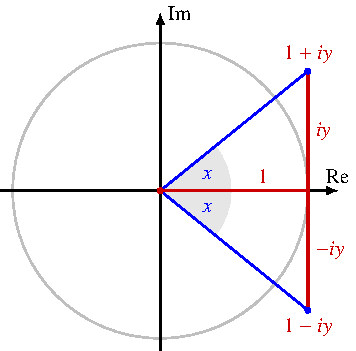
\includegraphics{chapters/070-intalg/images/invtan.pdf}
\caption{Bestimmung des Logarithmus bei der Berechnung des Arkustangens.
Der gesuchte Winkel ist der halbe Drehwinkel zwischen den Punkten
$1-iy$ und $1+iy$.
Der Quotient $(1-iy)/(1+ix)$ ist eine komplexe Zahl vom Betrag $1$ 
und daher von der Form $e^{2ix}$.
\label{buch:intalg:elementar:trigo:fig:invtan}}
\end{figure}
